\documentclass[12pt]{article}
\usepackage[utf8]{inputenc}
\usepackage[T1]{fontenc}
\usepackage{amsmath}
\usepackage{amsfonts}
\usepackage{amssymb}
\usepackage[version=4]{mhchem}
\usepackage{stmaryrd}
\usepackage{bbold}
\usepackage{hyperref}
\usepackage{graphicx}
\graphicspath{{../data/}}

\usepackage{listings} % Required for insertion of code
\usepackage{xcolor} % Required for custom colors

% Define custom colors
\definecolor{codegreen}{rgb}{0,0.6,0}
\definecolor{codegray}{rgb}{0.5,0.5,0.5}
\definecolor{codepurple}{rgb}{0.58,0,0.82}
\definecolor{backcolour}{rgb}{0.95,0.95,0.92}

% Setup the style for code listings
\lstdefinestyle{mystyle}{
    backgroundcolor=\color{backcolour},   
    commentstyle=\color{codegreen},
    keywordstyle=\color{magenta},
    numberstyle=\tiny\color{codegray},
    stringstyle=\color{codepurple},
    basicstyle=\ttfamily\footnotesize,
    breakatwhitespace=false,         
    breaklines=true,                 
    captionpos=b,                    
    keepspaces=true,                 
    numbers=left,                    
    numbersep=5pt,                  
    showspaces=false,                
    showstringspaces=false,
    showtabs=false,                  
    tabsize=2
}

% Activate the style
\lstset{style=mystyle}

\hypersetup{colorlinks=true, linkcolor=blue, filecolor=magenta, urlcolor=cyan,}
\urlstyle{same}

\title{Assignment 1: Exact diagonalization and quantum phase transitions }


\author{Instructor: Lesik Motrunich\\
TA: Liam O'Brien}
\date{}


\begin{document}
\maketitle
Ph 121C: Computational Physics Lab, Spring 2024

California Institute of Technology

Due: Tuesday, April 16, 2024

\section*{1 Introduction to quantum phase transitions}
In this assignment we will learn about the exact diagonalization method for quantum many-body physics and use it to investigate the phenomenon of quantum phase transitions in condensed matter systems. The analysis of phase transitions that occur at finite temperature should be familiar to you from statistical mechanics courses. These include transitions to superconductivity and superfluidity, as well as the transition to ferromagnetism at the Curie temperature. Generally speaking, a finite-temperature phase transition involves non-analyticity in some derivative of a system's free energy as a function of temperature. Continuous, or second-order, phase transitions fall into universality classes according to the power-law divergence of physical quantities like heat capacity and susceptibility, and the disappearance of the order parameter. All finite-temperature phase transitions are ultimately "classical," because above some length scale the phase change is primarily driven by thermal fluctuations.

Quantum phase transitions, instead, occur at $T=0$ as one varies the parameters of the Hamiltonian specifying the system, and are signified by qualitative changes in the nature of the ground state which are driven by purely quantum mechanical fluctuations. However, they inherit the phenomenology of continuous phase transitions: at the critical point, physical properties still develop singularities (in the thermodynamic limit) which allow us to define critical indices, and thus universality classes. The goal of this assignment is to provide you with experience in the phenomenology of phase transitions of quantum many-body Hamiltonians and to familiarize you with the exact diagonalization method for such problems. We will sometimes refer to a set of excellent lecture notes on the latter topic by Sandvik [1].

\section*{2 Quantum Ising model in one dimension}
\subsection*{2.1 Many-body Hilbert space}
Our example for this assignment is the quantum Ising model in one dimension. Consider a system living on a regular lattice of $L$ sites. At each site $j=1, \ldots, L$, we place a spin- $1 / 2$ degree of freedom (qubit), whose state is described by a vector in a 2-dimensional local Hilbert space $\mathcal{H}_{j}$. Each local Hilbert space is spanned by orthonormal basis vectors we denote $|\uparrow\rangle$ and $|\downarrow\rangle$, corresponding to spin up and down, respectively, in the $z$ direction. The local Hilbert space is a vector space over $\mathbb{C}$ having an inner product and standard norm, and a general (pure) state is of the form $\left|\psi_{j}\right\rangle=c_{\uparrow}|\uparrow\rangle+c_{\downarrow}|\downarrow\rangle$, where $c_{\uparrow, \downarrow} \in \mathbb{C}$ and $\left|c_{\uparrow}\right|^{2}+\left|c_{\downarrow}\right|^{2}=1$. The full many-body Hilbert spacecontaining all possible states of the chain - is described by a vector in a much larger space which has a simple decomposition: it is the $L$-fold tensor product of all of the local Hilbert spaces. That is, $\mathcal{H}=\mathcal{H}_{1} \otimes \mathcal{H}_{2} \otimes \cdots \otimes \mathcal{H}_{L} \cong\left(\mathbb{C}^{2}\right)^{\otimes L}$. A convenient orthonormal basis for $\mathcal{H}$ consists of the following vectors:


\begin{align*}
\left|e_{0}\right\rangle & \left.=\left|\uparrow_{1} \otimes\right| \uparrow\right\rangle_{2} \otimes|\uparrow\rangle_{3} \otimes \cdots \otimes|\uparrow\rangle_{L} \equiv\left|\uparrow_{1} \uparrow_{2} \uparrow_{3} \cdots \uparrow_{L}\right\rangle \\
\left|e_{1}\right\rangle & =\left|\downarrow_{1} \uparrow_{2} \uparrow_{3} \cdots \uparrow_{L}\right\rangle, \\
\left|e_{2}\right\rangle & =\left|\uparrow_{1} \downarrow_{2} \uparrow_{3} \cdots \uparrow_{L}\right\rangle,  \tag{1}\\
\left|e_{3}\right\rangle & =\left|\downarrow_{1} \downarrow_{2} \uparrow_{3} \cdots \uparrow_{L}\right\rangle, \\
& \vdots \\
\left|e_{2^{L}-1}\right\rangle & =\left|\downarrow_{1} \downarrow_{2} \downarrow_{3} \cdots \downarrow_{L}\right\rangle .
\end{align*}


Using this (or any other orthonormal) basis, the state of the system is written $|\psi\rangle=\sum_{\alpha=0}^{2^{L}-1} c_{\alpha}\left|e_{\alpha}\right\rangle$, where $c_{\alpha} \in \mathbb{C}$ for all $\alpha$ and $\sum_{\alpha}\left|c_{\alpha}\right|^{2}=1$. To see why the basis (1) is nice, relabel the local basis states as follows: $|\uparrow\rangle \mapsto|0\rangle,|\downarrow\rangle \mapsto|1\rangle$. Then the many-body basis states are $\left|e_{0}\right\rangle=|000 \cdots 0\rangle$, $\left|e_{1}\right\rangle=|100 \cdots 0\rangle,\left|e_{2}\right\rangle=|010 \cdots 0\rangle,\left|e_{3}\right\rangle=|110 \cdots 0\rangle$, and so on. Using this choice, the spin configuration of basis state $\alpha=0, \ldots, 2^{L}-1$ is found easily from the base- 2 representation of $\alpha$, with more significant bits toward the right ("little endian" order). As computers store integers in terms of their bits, to see the classical state of spin $j=1, \ldots, L$ in $\left|e_{\alpha}\right\rangle$ one need only read off the bit $j-1$ in the number $\alpha$, which can be done using fast bitwise operations 3. For example, in python or $\mathrm{C}$ the code alpha \& $1(\ll j-1)$ evaluates to 0 if $\operatorname{spin} j$ is in state $|\uparrow\rangle$, or to $2^{j-1}$ for $|\downarrow\rangle$.

Two important notions for many-body quantum systems are correlations and entanglement. These concepts will appear in this and subsequent assignments and will be used frequently to characterize quantum ground states and phases. For example, according to the above description, consider the following state which is perfectly valid for a three-site system:


\begin{equation*}
\left|\psi_{\mathrm{ex}}\right\rangle=\frac{\left|\uparrow_{1} \uparrow_{2} \uparrow_{3}\right\rangle+\left|\downarrow_{1} \downarrow_{2} \uparrow_{3}\right\rangle}{\sqrt{2}} . \tag{2}
\end{equation*}


It is evident that in such a state it is impossible to answer a question like, "is spin 1 pointing up or down?" Instead, we could conceivably ask, "what is the probability that spin 1 is pointing up?", as is often done in single-particle QM. But it turns out that this type of question is not very useful in the many-body context. More interesting probes account for the correlated nature of the state: for example, "how correlated is spin 1 with spin 2?" (to which the answer would be, perfectly) or "how correlated is spin 1 with spin 3?" (to which the answer is, not at all). This distinction manifests itself in the ability to usefully decompose the state (2) as follows:


\begin{equation*}
\left|\psi_{\text {ex }}\right\rangle=\frac{1}{\sqrt{2}}\left(\left|\uparrow_{1} \uparrow_{2}\right\rangle+\left|\downarrow_{1} \downarrow_{2}\right\rangle\right) \otimes\left|\uparrow_{3}\right\rangle \tag{3}
\end{equation*}


\subsection*{2.2 Hamiltonian}
The Hamiltonian of a quantum system is a linear operator acting on the Hilbert space $\mathcal{H}$. It implements a measurement of energy and also controls dynamics via the Schrödinger equation, and thermodynamic equilibrium of the quantum system. Only eigenstates of $\mathcal{H}$ have definite energy, and because the Hamiltonian also determines the time evolution of the system, energy eigenstates are stationary in time. Thus the energy eigenstates specify a preferred basis for $\mathcal{H}$. In particular, we will be mostly concerned with the ground state of $H$, which the system occupies with certainty in the zero-temperature limit due to the total suppression of thermal fluctuations.

The quantum Ising model is a generalization of the classical Ising model, and simulates the behavior of magnets by means of interactions in the $z$ components of neighboring spin- $1 / 2$ degrees of freedom, subject to an applied magnetic field in the transverse $x$ direction. The Hamiltonian on the one-dimensional chain of sites labeled $j=1, \ldots, L$ as described above is


\begin{equation*}
H=-J \sum_{j=1}^{L-1} \sigma_{j}^{z} \sigma_{j+1}^{z}-h \sum_{j=1}^{L} \sigma_{j}^{x} \tag{4}
\end{equation*}


Each $h$ or $J$ term is a Pauli spin matrix acting on the local Hilbert space of a particular site or a product of Paulis acting on two neighboring sites. As written here, the model has open boundary conditions. One can make the lattice periodic by adding the term $-J \sigma_{L}^{z} \sigma_{1}^{z}$, which we often do to mitigate boundary effects (we minimize finite-size effects because we are typically interested in the thermodynamic limit $L \rightarrow \infty$ ).

We have abused notation somewhat when writing the above lattice Hamiltonian. A priori, it does not make sense to take the sum of operators acting on different spaces, as written in (4). We have suppressed the trivial action of each operator on all other sites in the system, which is simply the identity in that local Hilbert space. That is,


\begin{align*}
\sigma_{j}^{x} & =\mathbb{I}_{1} \otimes \mathbb{I}_{2} \otimes \cdots \otimes \mathbb{I}_{j-1} \otimes \sigma_{j}^{x} \otimes \mathbb{I}_{j+1} \otimes \mathbb{I}_{j+2} \otimes \cdots \otimes \mathbb{I}_{L}  \tag{5}\\
\sigma_{j}^{z} \sigma_{j+1}^{z} & =\mathbb{I}_{1} \otimes \mathbb{I}_{2} \otimes \cdots \otimes \mathbb{I}_{j-1} \otimes \sigma_{j}^{z} \otimes \sigma_{j+1}^{z} \otimes \mathbb{I}_{j+2} \otimes \cdots \otimes \mathbb{I}_{L} \tag{6}
\end{align*}


with the natural definition of the tensor product of operators:


\begin{equation*}
(A \otimes B \otimes \ldots)(|v\rangle \otimes|w\rangle \otimes \ldots)=|A v\rangle \otimes|B w\rangle \otimes \ldots \tag{7}
\end{equation*}


That is, $\sigma_{j}^{x}$ can change the state of only the $j$-th spin. For example,


\begin{equation*}
\sigma_{j}^{x}\left|s_{1} s_{2} \ldots s_{j-1} \uparrow_{j} s_{j+1} \ldots s_{L}\right\rangle=\left|s_{1} s_{2} \ldots s_{j-1} \downarrow_{j} s_{j+1} \ldots s_{L}\right\rangle . \tag{8}
\end{equation*}


This notation, omitting operator tensor product symbols as well as identity operator factors, is clearly much more concise and is always used. Hamiltonians containing only terms of this form are described as " $k$-local," where $k$ is the maximum number of contiguous sites on which an individual term acts nontrivially (for example, (4) is 2-local). $k$-local Hamiltonians are the subject of widespread study, and are thought to be good approximations to many physical systems.

\subsection*{2.3 Ground states and phase transitions}
Often quantum phase transitions are the result of competing ground-state preferences dictated by the various types of terms in the Hamiltonian. This is easily seen in the Ising model (4). On the one hand, the $-J \sigma_{j}^{z} \sigma_{j+1}^{z}$ interaction terms minimize energy by aligning neighboring spins along the $z$-direction identically in either of the symmetry-breaking $|\uparrow \uparrow\rangle$ or $|\downarrow \downarrow\rangle$ states. On the other, the\\
$-h \sigma_{j}^{x}$ magnetic field terms minimize energy with spins oriented in the perpendicular $x$-direction, that is, the $|+\hat{x}\rangle=(|\uparrow\rangle+|\downarrow\rangle) / \sqrt{2}$ state. This state maintains the Ising spin-flip symmetry of the Hamiltonian. Thus, the relative strengths of $J$ and $h$ determine which type of state is the ground state.

In fact, the ground state wavefunction depends only on the ratio $h / J$, which attains a critical value $(h / J)_{c}=1$. In the quantum Ising model, for $h / J<(h / J)_{c}$ we expect a magnetically ordered phase, while for $h / J>(h / J)_{c}$ we expect a "disordered" phase (often called a quantum paramagnet). Approaching the critical point $(h / J)_{c}$ the correlation length of the ground state diverges, allowing quantum fluctuations at all length scales to take the system between the two phases. Accordingly, irrespective of the low-energy spectra of either phase around the transition, the excitation gap of the Hamiltonian vanishes at the critical point.

The ground state in the magnetically ordered phase is two-fold degenerate, roughly corresponding to the states $|\uparrow \uparrow \uparrow \cdots\rangle$ and $|\downarrow \downarrow \downarrow \cdots\rangle$. More precisely, there are two low-energy states with exponentially small splitting in system size, but these are actually linear combinations of the symmetry-breaking states. Any finite quantum system respects all of its symmetries; thus the true eigenstates are eigenstates of the Ising symmetry operator $U_{x}=\prod_{j} \sigma_{j}^{x}$, which are essentially $\frac{1}{\sqrt{2}}(|\uparrow \uparrow \uparrow \ldots\rangle \pm|\downarrow \downarrow \downarrow \ldots\rangle)$. All of these statements are correct in the limit $h / J \rightarrow 0$, and remain quite accurate elsewhere within the phase. The first excitation above this two-dimensional ground state manifold has a finite energy gap that persists in the thermodynamic limit.

In the paramagnetic phase, the ground state is non-degenerate. In this case, it is easier to describe, being simply the state $|+\hat{x}\rangle \otimes|+\hat{x}\rangle \otimes \cdots$ in the limit $h / J \rightarrow \infty$. Here again there is a finite energy gap to the excited state spectrum even for $L \rightarrow \infty$.

\subsection*{2.4 Observables}
To study the magnetic ordering within each phase and at the transition, we look for a quantity that behaves like an order parameter. The ground state expectation value of $M / L=\sum_{j=1}^{L} \sigma_{j}^{z} / L$ will be strictly zero in all phases due to the exact Ising symmetry of the Hamiltonian in finite systems. Instead, we can measure the expectation value of $(M / L)^{2}$ :


\begin{equation*}
\left\langle M^{2}\right\rangle=\sum_{j, k}\left\langle\sigma_{j}^{z} \sigma_{k}^{z}\right\rangle \xrightarrow{\text { p.b.c. }} L \sum_{r=0}^{L-1}\left\langle\sigma_{1}^{z} \sigma_{1+r}^{z}\right\rangle . \tag{9}
\end{equation*}


In the second step we use the translation invariance of the system under periodic boundary conditions to reduce the complexity of computing this quantity. In the ferromagnetic phase, $\left\langle(M / L)^{2}\right\rangle$ will saturate to a constant, but will decrease to zero (somewhat weakly) with system size $L$ in the paramagnetic phase, providing a quantitative distinction.

Rather than calculating $\left\langle M^{2}\right\rangle$, it is actually more instructive to study the correlation function $C^{z z}(r) \equiv\left\langle\sigma_{1}^{z} \sigma_{1+r}^{z}\right\rangle$ which is used in the second definition above. The asymptotic scaling of $C^{z z}(r)$ displays a characteristic form which is indicative of the phase: namely, the persistence of a strictly non-zero value even for $r \rightarrow \infty$ which identifies the magnetically ordered phase, contrasted with exponential decay to zero in the disordered phase. In addition, the decay of the correlation function takes a different form at the critical point itself, a fact which is closely related to the closing of the excitation gap (this topic is investigated in Sec. 4.6). From the scaling of the correlation function one can define another order parameter given by $\sqrt{\left\langle\sigma_{1}^{z} \sigma_{L / 2}^{z}\right\rangle}$, which provides a single quantity which either saturates or monotonically decreases with increasing system size, corresponding to the presence or absence of magnetic order. (Note that in a periodic system the longest distance is $L / 2$ because correlations can develop going in either direction on the chain, which is a circle.)

\section*{3 Exact diagonalization of many-body Hamiltonians}
Exact diagonalization (ED) is a numerical method which entails constructing an explicit representation of the Hamiltonian operator in the Hilbert space $\mathcal{H}$, which one can diagonalize using standard numerical linear algebra tools. The primary advantage of ED is that it can be applied to any system in essentially the same way. The impediment to using ED is that it quickly becomes infeasible due to the exponential growth in dimension of the Hilbert space of a many-body system.

\subsection*{3.1 Dense diagonalization methods}
The most straightforward approach to ED is to simply represent the entire Hamiltonian as a dense matrix. To do so requires storing $\operatorname{dim}(\mathcal{H})^{2}=\left(2^{L}\right)^{2}$ elements, a cost which quickly becomes prohibitive: already for $L=16, H$ requires $34 \mathrm{~GB}$ of memory in double precision floats. In order to explicitly generate the Hamiltonian one can simply compute all $\left(2^{L}\right)^{2}$ matrix elements as $H_{\alpha \beta} \equiv\left\langle e_{\alpha}|H| e_{\beta}\right\rangle$ using, e.g., the mapping from spin configurations to basis states described in (1). The Hermiticity of $H\left(H_{\beta \alpha}=H_{\alpha \beta}^{*}\right)$ can reduce the memory cost by a factor of roughly 2 . One can also use diagonalization routines optimized for Hermitian matrices, or for real symmetric matrices if all matrix elements $H_{\alpha \beta}$ are real, which significantly improves algorithmic performance.\\

\subsection*{3.2 Sparse matrix representation}
Written in the basis (1), nearly all of the matrix elements of $H$ will turn out to be 0 . To understand this, consider the structure of the terms comprising the Hamiltonian, described in Sec. 2.2. Only very specific types of states are connected by each of the local terms. Consider, for example, $\sigma_{j}^{z} \sigma_{j+1}^{z}$, whose explicit form is shown in (6). To have a nonzero matrix element for this term, two basis states $\left|e_{\alpha}\right\rangle$ and $\left|e_{\beta}\right\rangle$ must be identical on all sites where the operator acts trivially, in order to be connected by all $L-2$ identities $\mathbb{I}_{k}, k \neq j, j+1$. Because $\sigma_{j}^{z} \sigma_{j+1}^{z}$ acting in the local Hilbert space is also diagonal, it connects only basis states which are identical on all sites including $j$ and $j+1$, but with the crucial addition of a sign to the matrix element for certain two-spin configurations:

\[
\sigma_{j}^{z} \sigma_{j+1}^{z}=\mathbb{I}_{1} \otimes \cdots \otimes \mathbb{I}_{j-1} \otimes\left[\begin{array}{cccc}
1 & 0 & 0 & 0  \tag{10}\\
0 & -1 & 0 & 0 \\
0 & 0 & -1 & 0 \\
0 & 0 & 0 & 1
\end{array}\right]_{j, j+1} \otimes \mathbb{I}_{j+2} \otimes \cdots \otimes \mathbb{I}_{L}
\]

On the other hand, because the $\sigma_{j}^{x}$ matrix is off-diagonal in this basis, these terms connect states related by a single spin-flip. Consider the state $\left|e_{\beta}\right\rangle$ : we can ask with which state it has nonzero matrix element $\left\langle e_{\alpha}\left|\sigma_{j}^{x}\right| e_{\beta}\right\rangle$. One can quickly obtain $\alpha$ by using the bitwise XOR operation to flip the $j$ th bit in the stored binary representation of $\beta$.

Evidently, the Hamiltonian in this basis is more appropriately represented as a sparse matrix, avoiding having to store and manipulate an overwhelming number of zeros. A local Hamiltonian like $H$ has roughly $L \times 2^{L}$ nonzero terms, an enormous reduction compared with $\left(2^{L}\right)^{2}$. One can represent the sparse matrix by identifying the basis states connected by each term in $H$ and

tabulating all 3 -tuples $\left(\alpha, \beta, H_{\alpha \beta}\right)$ of nonzero matrix elements. The challenge of the sparse matrix approach lies predominantly in creating a bookkeeping system for all of the basis states and correctly identifying every nonzero matrix element of $H$.

There is no single standard format for sparse matrix representation. The table of triplets described above is known as "COO" format and is often convenient for initialization but inefficient when used in numerical routines. A common design pattern is to initialize a sparse matrix in COO\\
format, then convert it to a more computationally friendly option before calling a diagonalization routine. Ultimately one needs to consult the relevant documentation, e.g., Ref. [4].

\subsection*{3.3 Lanczos method}
With this improvement in storage, we can tackle significantly larger systems, but of course the difficulty of computing the eigenstates continues to increase with the system size. It becomes impossible to solve for the entire spectrum of a sparse matrix while maintaining the improved storage, but one can find a few eigenstates at either end of the spectrum or, with some more effort, from somewhere in the middle via "shift-and-invert" methods. A variety of iterative schemes exist, but they are not nearly as clean and robust as dense diagonalization. In particular, matrices with high condition number (the ratio of the largest-magnitude eigenvalue to the smallest) may present difficulties with convergence. One state-of-the-art sparse diagonalization library is ARPACK, which is written in Fortran but has interfaces in Python and Julia, and several in C++.

The algorithm generally favored in physics applications is one devised by Lanczos as an improvement over the basic power method. The power method is based on the observation that a random initial state $|\psi\rangle$ can be decomposed in the eigenbasis of $H$, and, if $H$ is applied to $|\psi\rangle$, the component in the direction of the leading eigenvector of $H$ (i.e., having the eigenvalue of largest magnitude) will increase relative to the other eigenvectors having eigenvalues of smaller magnitude. That is, if $H=\sum_{\alpha} \epsilon_{\alpha}\left|v_{\alpha}\right\rangle\left\langle v_{\alpha}\right|$ and $|\psi\rangle=\sum_{\alpha} c_{\alpha}\left|v_{\alpha}\right\rangle$,


\begin{equation*}
H|\psi\rangle=\sum_{\alpha} \epsilon_{\alpha} c_{\alpha}\left|v_{\alpha}\right\rangle, \quad \text { and } \frac{\left|\epsilon_{1} c_{1}\right|^{2}}{\sum_{\alpha>1}\left|\epsilon_{\alpha} c_{\alpha}\right|^{2}}>\frac{\left|c_{1}\right|^{2}}{\sum_{\alpha>1}\left|c_{\alpha}\right|^{2}} \tag{11}
\end{equation*}


with the eigenvalues sorted so that $\left|\epsilon_{1}\right|>\left|\epsilon_{\alpha}\right|$ for all $\alpha>1$. This also requires that the leading eigenvector be unique. The power method can be described recursively by $\left|\psi_{k+1}\right\rangle=H\left|\psi_{k}\right\rangle / \| H\left|\psi_{k}\right\rangle||$, which in the limit $k \rightarrow \infty$ converges to the extremal eigenvector. (This is the same argument made to claim the dominance of the maximal eigenvector of the transfer matrix in the thermodynamic limit of a 1d stat mech model.) However, in practice the convergence of this method turns out to be extremely slow, and its performance strongly depends on the gap to the first excited state.

Because up to normalization the power method is simply the application of $H^{k}$ - the $k$-th power of the Hamiltonian - to an arbitrary state, one might wonder whether instead any degree $k$ polynomial of the Hamiltonian could be found having superior convergence, with no extra work since we already compute $H^{l}|\psi\rangle$ for $0 \leq l \leq k$. The span of these states in $\mathcal{H}$ is called the Krylov subspace, and the Lanczos algorithm entails finding the basis within this subspace that simplifies $H$ as much as possible. For a precise description of the basic Lanczos method including pseudocode, see Sandvik's lecture notes, Ref. [1], or the textbook by Golub and van Loan, Ref. [2].

In this assignment you are not required to implement your own Lanczos algorithm and will make use of some standard sparse matrix library. However, if you are interested in this type of calculation, writing your own is an instructive experience. One further algorithmic simplification (described also by Sandvik) removes the necessity of directly representing the Hamiltonian at all. It turns out the Lanczos algorithm does not even need to know $H$ : it's only necessary to be able to perform $|\psi\rangle \mapsto H|\psi\rangle$. Thus, most implementations allow you to provide a function pointer that computes the application of $H$ to a vector rather than supplying a sparse matrix in any format. Using such a matrix-free specification of the Hamiltonian can be even more efficient.

\subsection*{3.4 Restriction to symmetry sectors}
Global symmetries of a Hamiltonian can be used to reduce the effort required for ED, in some cases drastically. Here we discuss implementation of the global symmetry of the Ising model by again considering the states connected to each other by the Hamiltonian, as in Sec. 3.2.

The Ising symmetry operator is $U_{x}=\prod_{j} \sigma_{j}^{x}$, with eigenvalues $\pm 1$. Accordingly, the total Hilbert space decomposes into the direct sum of the corresponding eigenspaces $\mathcal{H}=\mathcal{H}_{-} \oplus \mathcal{H}_{+}$. Since $U_{x}$ commutes with $H$, the Hamiltonain preserves (i.e., acts without mixing) $\mathcal{H}_{-}$and $\mathcal{H}_{+}$. It is easiest to access these eigenspaces by performing a basis rotation, from the $\sigma^{z}$ eigenstates in (1), which use local $|\uparrow\rangle$ and $|\downarrow\rangle$ basis, to the $\sigma^{x}$ basis built from states we denote $|+\rangle=|+\hat{x}\rangle$ and $|-\rangle=|-\hat{x}\rangle$.

The accounting of the states that you have already done can be used as-is, as so far this is only a trivial relabeling. The distinction comes in the explicit form of the terms in the Hamiltonian (4), which no longer have the matrix elements described in Sec. 3.2. Instead, one finds that $\sigma_{j}^{x}$ is diagonal in this basis (which is indeed why we chose it), and $\sigma_{j}^{z}$ is a spin-flip operator. Thus, the Hamiltonian connects states that either have the same number of $|+\rangle$-spins and $|-\rangle$-spins, or differ by two. $U_{x}$ counts the parity, and odd- and even-parity sectors are not connected by $H$.

The reduction of the Hilbert space is accomplished by separating the basis states according to their parity. Then one can set up an "odd" sector problem and an "even" sector problem by restricting the basis, each having Hilbert space dimension reduced by a factor of two. The energy eigenvalues in each sector will match those found in the full Hilbert space, with wavefunctions that are related by a unitary rotation. Because the cost of typical dense diagonalization routines scales as $O\left(N^{3}\right)$ in the linear dimension $N$ of the matrix, reducing $N$ by half obtains an eightfold speedup, which gives a fourfold overall reduction (as the routine must run twice).

\section*{4 Assignment: ED study of quantum Ising model}
For simplicity, in the following we set the parameter $J=1$ in (4) and vary $h$.

\subsection*{4.1 Dense ED}
Generate the quantum Ising Hamiltonian (4) as a dense matrix and call an explicit diagonalization routine for the entire spectrum for system sizes $L=8,10,12,14$, and for a range of values of $h$. Plot the ground state energy as a function of $h$ for the various $L$. Compare the open systems with periodic ones for the same parameters - how does each phase react to the boundaries?

\subsubsection{}

\begin{figure}
\centering
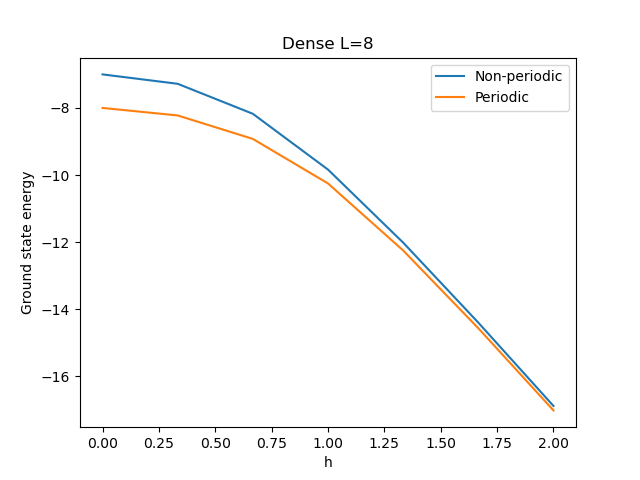
\includegraphics[width=0.75\textwidth]{dense_ising_model_L8.png}
\end{figure}

\begin{figure}
\centering
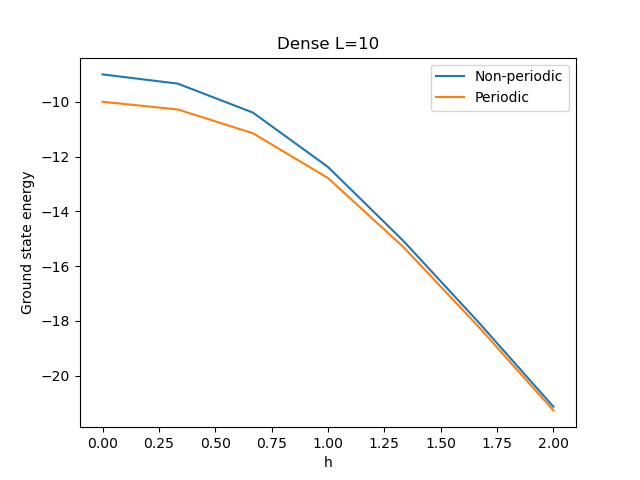
\includegraphics[width=0.75\textwidth]{dense_ising_model_L10.png}
\end{figure}

\begin{figure}
\centering
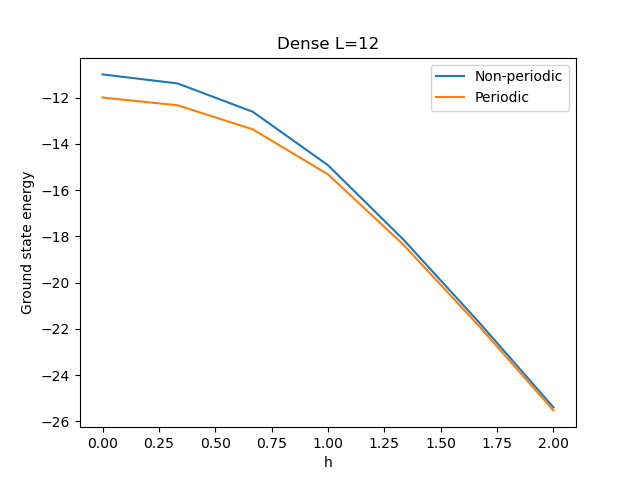
\includegraphics[width=0.75\textwidth]{dense_ising_model_L12.png}
\end{figure}

\begin{figure}
\centering
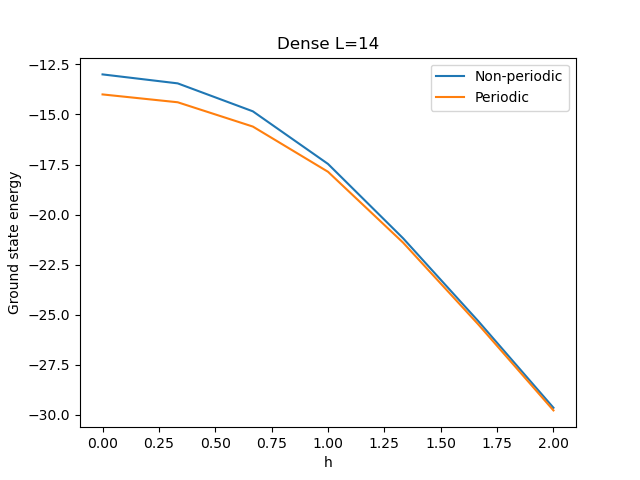
\includegraphics[width=0.75\textwidth]{dense_ising_model_L14.png}
\end{figure}

The paramagnetic phase (with the larger h value) does not care whether the boundaries are open or periodic because the assortment of spins is random and ways. For the ferromagnetic phase, there is a clear preference for the periodic boundary conditions, because this allows for an extra interaction term that minimizes the total energy even more.

% Inline Python code in the document
\begin{lstlisting}[language=Python]
sigma_x = np.array([[0, 1], [1, 0]])
sigma_z = np.array([[1, 0], [0, -1]])
I = np.identity(2)

def tensor_product(matrices):
    """Calculate the tensor product of a list of matrices."""
    result = matrices[0]
    for matrix in matrices[1:]:
        result = np.kron(result, matrix)
    return result

def open_dense_hamiltonian_explicit(L, h, J=1):
    # Initialize Hamiltonian to zero matrix
    H = np.zeros((2**L, 2**L))
    
    # Interaction term
    for i in range(L - 1):  # Add periodic term at the end if periodic
        matrices = [I] * L  # Start with identity matrices
        matrices[i] = sigma_z  # Apply sigma_z at position i
        matrices[(i + 1)] = sigma_z  # Apply sigma_z at position (i+1) modulo L for periodic
        H += -J * tensor_product(matrices)
    
    # Transverse field term
    for i in range(L):
        matrices = [I] * L  # Start with identity matrices
        matrices[i] = sigma_x  # Apply sigma_x at position i
        H += -h * tensor_product(matrices)
    
    return H

def periodic_dense_hamiltonian_explicit(L, h, J=1):
    # Initialize Hamiltonian to zero matrix
    H = np.zeros((2**L, 2**L))
    
    # Interaction term
    for i in range(L):  # Add periodic term at the end if periodic
        matrices = [I] * L  # Start with identity matrices
        matrices[i] = sigma_z  # Apply sigma_z at position i
        matrices[(i + 1) % L] = sigma_z  # Apply sigma_z at position (i+1) modulo L for periodic
        H += -J * tensor_product(matrices)
    
    # Transverse field term
    for i in range(L):
        matrices = [I] * L  # Start with identity matrices
        matrices[i] = sigma_x  # Apply sigma_x at position i
        H += -h * tensor_product(matrices)
    
    return H

L = [8, 10, 12, 14]
h_range = np.linspace(0, 2, 7)  # Generates 8 values of h from 0 to 2

for l in L:
    plt.figure()
    plt.title(f'Dense L={l}')
    open_ground_state_energies = []  # To store ground state energies for different h
    periodic_ground_state_energies = []  # To store ground state energies for different h
    for hi in h_range:
        # for the given hi, comupte gs energy for both periodic and non-periodic
        H = open_dense_hamiltonian_explicit(l, hi)
        print(f'H: hi={hi}\n{H}')
        H_periodic = periodic_dense_hamiltonian_explicit(l, hi)
        # Compute the ground state energy using the lowest eigenvalue
        open_ground_state_energies.append(min(np.linalg.eigvalsh(H)))
        periodic_ground_state_energies.append(min(np.linalg.eigvalsh(H_periodic)))
    # plot the ground state energy as a function of h for both periodic and non-periodic
    plt.plot(h_range, open_ground_state_energies, label='Non-periodic')
    plt.plot(h_range, periodic_ground_state_energies, label='Periodic')
    plt.xlabel('h')
    plt.ylabel('Ground state energy')
    plt.legend()
    # save a tout for the given value of L
    plt.savefig(f'dense_ising_model_L{l}.png')
\end{lstlisting}



\subsection*{4.2 Sparse ED}
Construct the same Hamiltonian as a sparse matrix and use a sparse matrix diagonalization routine provided by a standard library. Obtain the ground state and a few excited states, and for small system sizes verify your results against the dense ED solution. How large of a system can you push the sparse diagonalization routine to solve?


Optional. Try implementing your own Lanczos routine.
\subsubsection{}
As can be seen from the plot, the energies for the GS and first excited states are identical for the L=10 and L=12 systems.
\begin{figure}
\centering
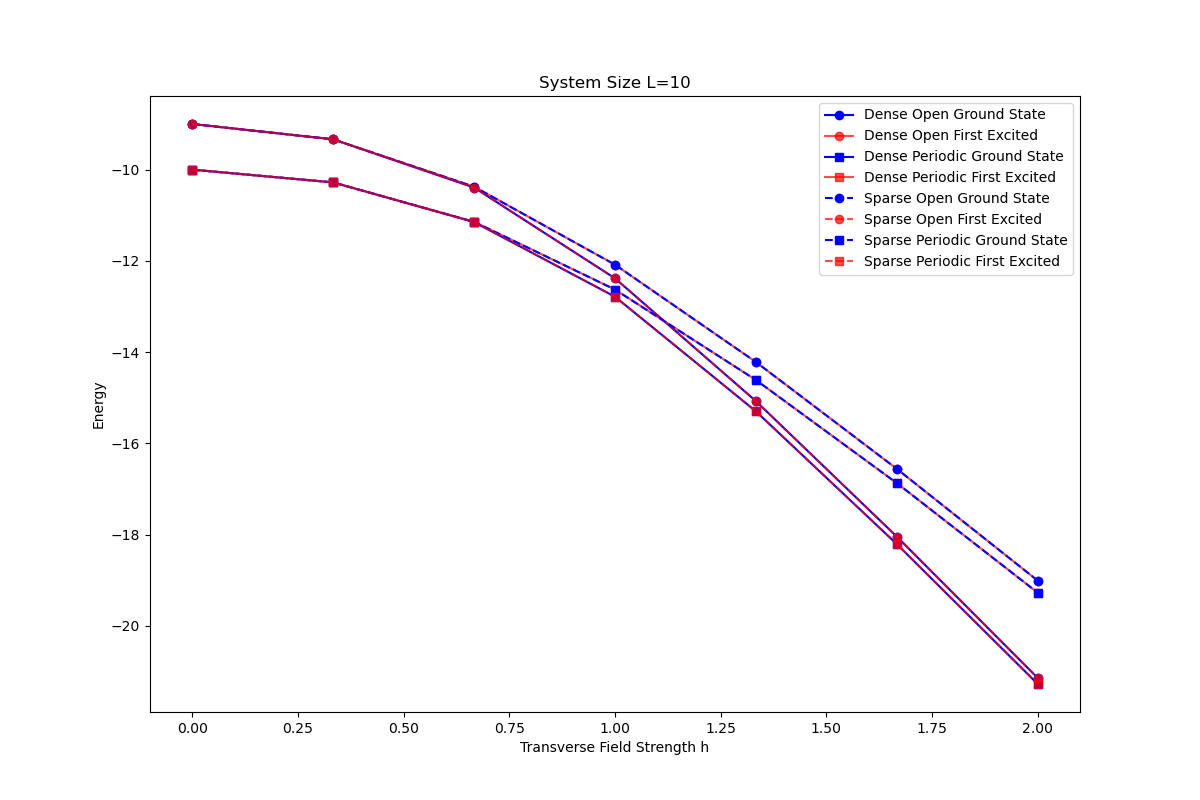
\includegraphics[width=\textwidth]{enhanced_compare_ising_model_L10.png}
\end{figure}

\begin{figure}
\centering
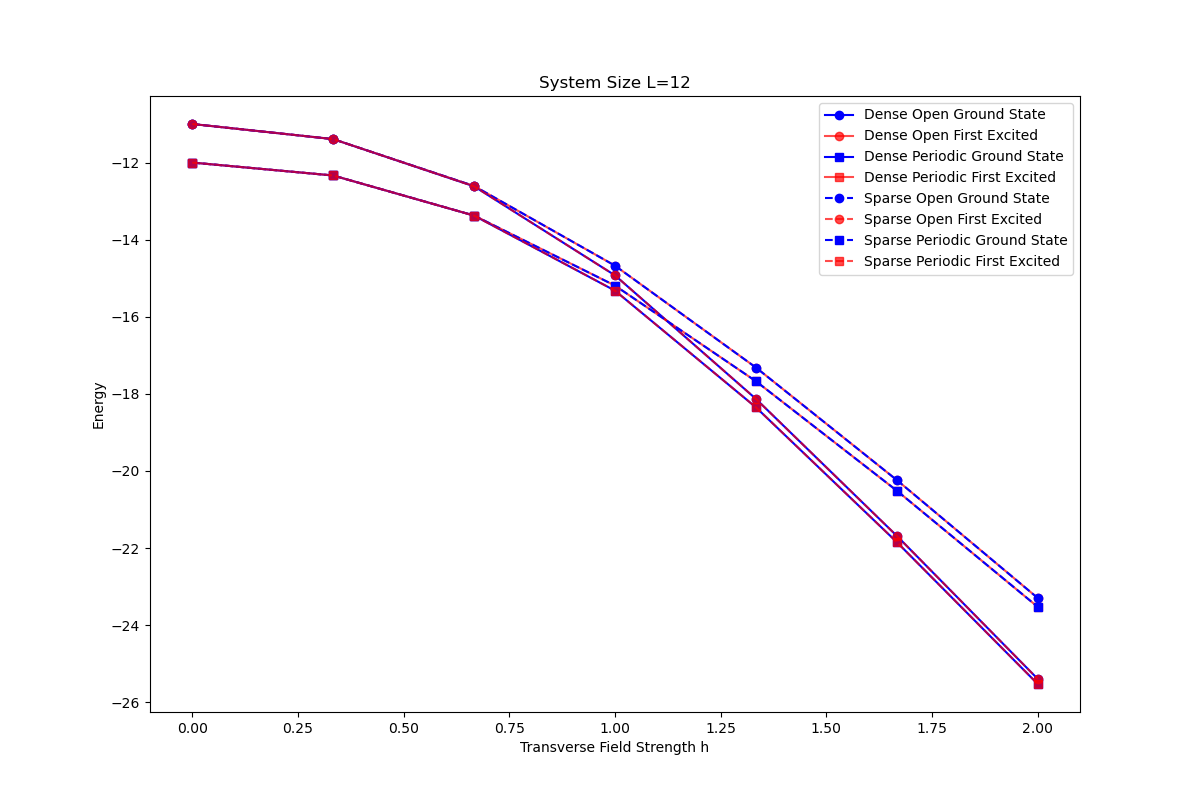
\includegraphics[width=\textwidth]{enhanced_compare_ising_model_L12.png}
\end{figure}

% Inline Python code in the document
\begin{lstlisting}[language=Python]
def sparse_hamiltonian(L, h, J=1, periodic=False):
    row = []
    col = []
    data = []
    # loop over the index i
    for i in range(2**L):
        # turn that index into a binary string
        bi = binary_string(i, L)

        # to the diagonal element first
        total_interaction = 0
        # initialize the loop range based on the boundary conditions
        loop_range = L if periodic else L - 1
        for k in range(loop_range):
            # Handle periodic boundary by wrapping the index
            next_k = (k + 1) % L if periodic else k + 1
            # Add neighbor interaction based on the spin values
            total_interaction += -J * (1 if bi[k] == bi[next_k] else -1)
        row.append(i)
        col.append(i)
        data.append(total_interaction)

        # now consider the off-diagonal elements connected by a single spin flip
        # make a function that takes the bit i and returns a list of basis states connected by a single flip
        def flip(i):
            connected_bases_states = []
            for j in range(L):
                flip_i = i ^ (1 << j)
                connected_bases_states.append(flip_i)
            return connected_bases_states
        
        # loop over the connected basis states
        for flip_i in flip(i):
            row.append(i)
            col.append(flip_i)
            data.append(-h)       

    # Create a sparse matrix from the lists
    H = scipy.sparse.coo_matrix((data, (row, col)), shape=(2**L, 2**L))
    return H
\end{lstlisting}



\subsection*{4.3 Study of convergence with system size}
For representative values of $h$ inside each phase (e.g., $h=0.3$ in the ferromagnetic phase and $h=1.7$ in the paramagnet), study the $L$ dependence of the ground state energy per site, $E_{\mathrm{gs}}(L) / L$, for systems with both periodic and open boundary conditions. Comment on the approach to the thermodynamic limit $L \rightarrow \infty$ for the two types of boundaries.



It should be clear that periodic boundaries are preferred in order to minimize finite-size effects. However, sometimes open boundary conditions are preferred for technical reasons. An important example is the tensor network representation we will implement later in the course. One can mitigate the effects of the boundaries and better estimate the bulk energy per site using the following trick: for the system with open boundary conditions, plot the values $[E(L=10)-E(L=8)] / 2$, $[E(L=12)-E(L=10)] / 2$, etc. These quantities can be thought of as ground state energy per site for the two sites added in the middle, which feel reduced boundary effects.
\subsubsection{}
\begin{figure}
\centering
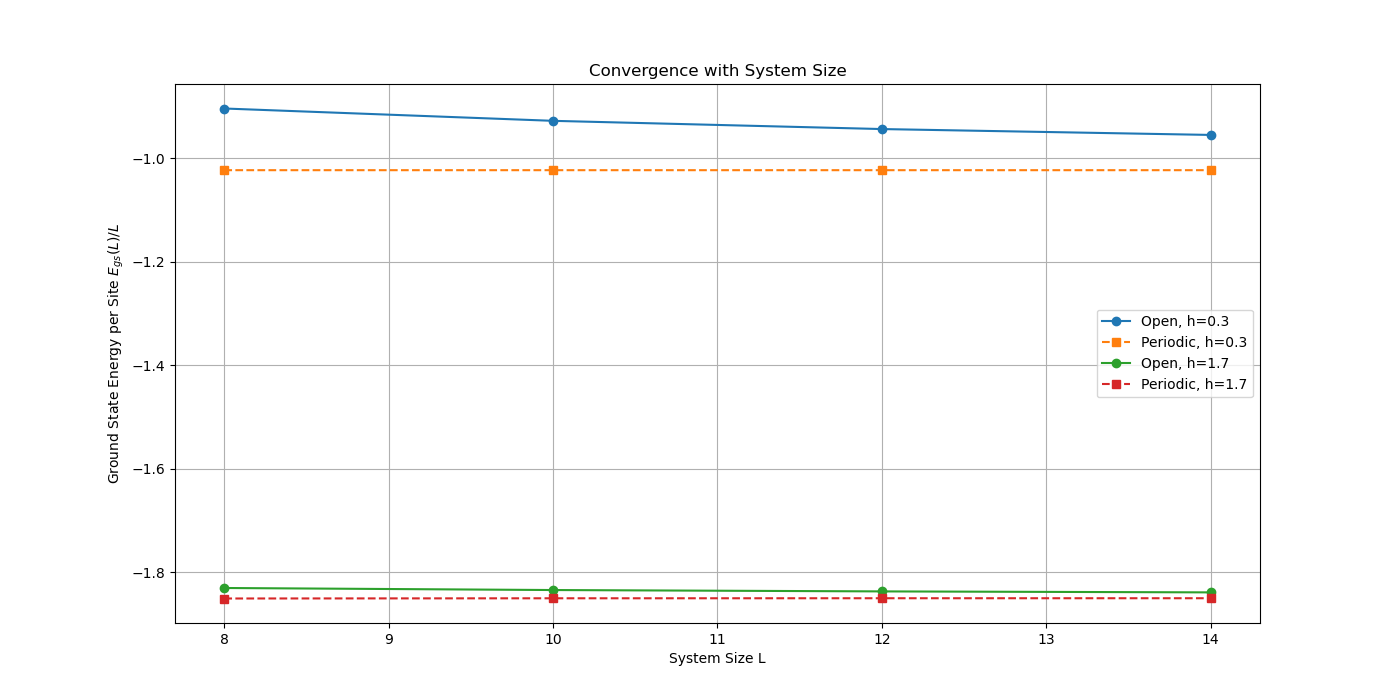
\includegraphics[width=\textwidth]{convergence.png}
\end{figure}

Both type of boundaries approach a thermodynamic limit as the system size increases. That is, the periodic systems should be more accurate, but this doesn't matter so much in the thermodynamic limit. One also notices that when we have a small transverse field $h$, the interaction terms dominatet, so the fined size effect is quite pronounced, but this is not the case when we have the larger value for $h$.

\subsection*{4.4 Finding the quantum phase transition}
From now on, consider only the chain with periodic boundary conditions. The quantum phase transition can be identified via the closing of the energy gap, as described in Sec. 2.3. Using the sparse eigensolver, plot the excitation energies (relative to the ground state) for a few excited states vs. $h$ for your largest system size. Estimate the critical field $h_{c}$ from this study and compare with the known value of $h_{c}=1$. The excitation gap is expected to vanish as $\Delta \sim\left|h-h_{c}\right|^{\nu}$. Can you determine the exponent $\nu$ from your data?

Another straightforward technique to find the phase transition is by studying so-called "fidelity." As you scan $h$, calculate the overlap between the ground states at consecutive $h$ and $h+\delta h$ and plot the fidelity $\left|\left\langle\psi_{\mathrm{gs}}(h) \mid \psi_{\mathrm{gs}}(h+\delta h)\right\rangle\right|$ as a function of $h$. Deep inside either phase, the character of the ground state changes little with changing $h$, and the fidelity is close to 1 . However, near the transition the character of the ground state changes rapidly and the fidelity exhibits a cusp. The peak height you observe will depend on $\delta h$.

\subsection*{4.5 Study of magnetic ordering}
One can also use the wavefunctions obtained from diagonalization to measure any observable in the ground state. For representative points in the two phases and also at the critical point, plot $C^{z z}(r)$ as defined in Sec. 2.4 as a function of $r$ for multiple system sizes $L$ and comment on the behavior at large separation $r$. Also compute the quantity $\left\langle(M / L)^{2}\right\rangle$ and compare the behavior of this order parameter with the half-chain correlation function values.

\subsection*{4.6 Optional. Study of critical correlations}
Measure the correlator $C^{x x}(r)=\left\langle\sigma_{1}^{x} \sigma_{1+r}^{x}\right\rangle$ as a function of $r$ in the ground state of both phases. Observe the long-distance behavior of this quantity; is it what you would have expected based on the discussion of Sec. 2.4. Why do you think you obtained this result?

For correlation functions such as the above, it is useful to instead study the connected correlator $C_{\text {conn }}^{x x}(r) \equiv\left\langle\sigma_{1}^{x} \sigma_{1+r}^{x}\right\rangle-\left\langle\sigma_{1}^{x}\right\rangle\left\langle\sigma_{1+r}^{x}\right\rangle$, which ignores the classical correlations between the two operators. The connected correlations display quasi-long range order at the critical point, meaning that they decay algebraically as a power law with distance. The set of exponents of these power laws is an inherent property of the critical theory. Try to fit the decay of the connected correlations at the critical point to a power-law form and extract the critical exponent associated with $C_{\operatorname{conn}}^{x x}(r)$. Importantly, because you are studying a relatively small periodic system, you will need to plot

$C_{\text {conn }}^{x x}(r)$ against the chord length $\left|\frac{L}{\pi} \sin \left(\frac{\pi r}{L}\right)\right|$ instead of simply $r$. Repeat this process for $C_{\text {conn }}^{z z}(r)$, extracting this critical exponent as well.

\subsection*{4.7 Making use of Ising symmetry}
In the previous steps, no use has been made of the Ising symmetry: the fact that unitary $U_{x}=\prod_{j} \sigma_{j}^{x}$ commutes with the Hamiltonian. Correctly implementing the symmetry reduces the size of the diagonalization problem by a factor of two, which saves memory and gives a fourfold speedup.

Set up a sparse diagonalization of the Ising Hamiltonian in the $\sigma^{x}$ basis, utilizing the Ising symmetry as described in Sec. 3.4. As you will no longer be able to exploit the convenient basis (1), the bookkeeping is more challenging here. Obtain a few states in each sector and compare with your previous results. Use the symmetric solver to add a single site to the largest size you were able to solve previously and find the ground state and a few excited states at this size for representative values of $h$ in each phase.

Utilizing symmetries can also improve the accuracy of certain interesting features of the spectrum. For example, in Sec. 2.3 the two ground states in the ordered phase are described as having an energy splitting that is exponentially small in system size. By solving for the ground state within each symmetry sector, try to obtain the dependence of this splitting on system size $L$.

\section*{5 Optional. Heisenberg antiferromagnetic chain}
The Heisenberg model also simulates the magnetic behavior of spin- $1 / 2$ degrees of freedom on a lattice, but with perhaps a more realistic spin-spin term adding $\sigma^{x}-\sigma^{x}$ and $\sigma^{y}-\sigma^{y}$ interactions to that of the Ising model. Here we do not apply the transverse magnetic field. The quantum Heisenberg Hamiltonian is


\begin{equation*}
H=J \sum_{j=1}^{L-1} \boldsymbol{\sigma}_{j} \cdot \boldsymbol{\sigma}_{j+1}=J \sum_{j=1}^{L-1}\left(\sigma_{j}^{x} \sigma_{j+1}^{x}+\sigma_{j}^{y} \sigma_{j+1}^{y}+\sigma_{j}^{z} \sigma_{j+1}^{z}\right) \tag{12}
\end{equation*}


This model has a continuous $\mathrm{O}(3)$ spin-rotation symmetry (because $H$ is symmetric in the $x, y$, and $z$ directions, we may rotate however we want in this 3 -dimensional space and the theory is invariant), so one might expect that the model hosts gapless degrees of freedom. This is correct, but we owe to Haldane the surprising discovery that if the local degrees of freedom have integer total spin, the ground state of $H$ is actually gapped.

\subsection*{5.1 Diagonalization within sectors of fixed $S_{\text {tot }}^{z}$}
For the purposes of numerical solution, the Heisenberg model has a very useful symmetry, which is conservation of total spin in the $z$-direction: $S_{\mathrm{tot}}^{z}=\sum_{j} S_{j}^{z}$. It is not immediately evident that this operator commutes with the Hamiltonian (12). To make the symmetry manifest, one rewrites the exchange interaction term using the spin-raising and lowering operators $S_{j}^{+}$and $S_{j}^{-}$, where


\begin{equation*}
2 S_{j}^{ \pm}=\sigma_{j}^{x} \pm i \sigma_{j}^{y} \tag{13}
\end{equation*}


Then $S^{+}|\uparrow\rangle=0, S^{+}|\downarrow\rangle=|\uparrow\rangle$, and $S^{-}|\uparrow\rangle=|\downarrow\rangle, S^{-}|\downarrow\rangle=0$. Some algebra demonstrates that


\begin{equation*}
2\left(S_{j}^{+} S_{j+1}^{-}+S_{j}^{-} S_{j+1}^{+}\right)=\sigma_{j}^{x} \sigma_{j+1}^{x}+\sigma_{j}^{y} \sigma_{j+1}^{y} . \tag{14}
\end{equation*}


Replacing the terms in the Hamiltonian (12) gives a form which manifestly commutes with $S_{\text {tot }}^{z}$. (As an aside, this is also the first step in the famous Jordan-Wigner transformation, which maps these qubit degrees of freedom to interacting spinless fermions hopping on a one-dimensional wire.)

Contrary to the case of the Ising model, here the $\sigma^{z}$ basis is appropriate for implementation of the symmetry. Additionally, there are many more eigenvalues of $S_{\text {tot }}^{z}$, and the dimension of each\\
eigenspace is greatly reduced, by about a factor of $L$. Solving for the ground state in multiple selection sectors gives a straightforward way of computing more diverse excited states than would otherwise be possible. However, in this example the bookkeeping required when identifying basis states of the full Hilbert space with those specific to a particular sector is more detailed than in the comparatively simple Ising case. To check your solutions, compare your results against a simpler setup that does not use $S^{z}$ conservation. The reduction of the dimension of the Hilbert space greatly increases the performance of the eigensolver and will allow you to reach yet larger system sizes. (You can simply set $J=1$ here, and the Hamiltonian 12 has no parameters.)

\section*{$5.2 \quad J_{1}-J_{2}$ Heisenberg chain}
One can modify the Heisenberg model to include second-neighbor interactions,


\begin{equation*}
H=J_{1} \sum_{j} \boldsymbol{\sigma}_{j} \cdot \boldsymbol{\sigma}_{j+1}+J_{2} \sum_{j} \boldsymbol{\sigma}_{j} \cdot \boldsymbol{\sigma}_{j+2} \cdot \tag{15}
\end{equation*}


This model undergoes a transition from a gapless "Bethe" phase to a gapped so-called "valence bond solid" (VBS) phase that spontaneously breaks the translational symmetry. Roughly, spins pair up into singlets on either the even or the odd links of the lattice. Such singlets are similar to chemical valence bonding, and the "bonds" form a crystal, hence the name VBS. The transition happens at $J_{2} / J_{1} \approx 0.25$, while $J_{2} / J_{1}=\frac{1}{2}$ is the special Majumdar-Ghosh point, where the above qualitative picture for the ground state is quantitatively exact.

One can apply similar techniques to find and characterize the transition as in the previous examples (e.g., monitor fidelity and observe opening of the gap as one varies $J_{2} / J_{1}$; study spinspin correlation functions and observe power law decay in the Bethe phase as compared with exponential decay in the VBS phase). One can also devise an order parameter for detecting VBS: $\sum_{j}(-1)^{j}\left\langle\boldsymbol{\sigma}_{j} \cdot \boldsymbol{\sigma}_{j+1}\right\rangle$ will roughly detect the "wave" at wavevector $\pi$ in the energy density of the valence bond crystal.

\section*{References}
[1] Sandvik, Anders W. "Computational studies of quantum spin systems." In AIP Conference Proceedings, vol. 1297, no. 1, pp. 135-338. American Institute of Physics, 2010.

[2] Golub, Gene H., and Charles F. van Loan. Matrix computations. Vol. 3. JHU press, 2013.

[3] \href{https://en.wikipedia.org/wiki/Bitwise_operation}{https://en.wikipedia.org/wiki/Bitwise\_operation}

[4] \href{https://docs.scipy.org/doc/scipy/reference/sparse.html}{https://docs.scipy.org/doc/scipy/reference/sparse.html}


\end{document}